\documentclass[11pt,english]{article}

\usepackage[utf8]{inputenc}
\usepackage[T1]{fontenc}

\usepackage[
  margin=1.3in,
  headheight=14pt]{geometry}


\usepackage{mathpazo}
\usepackage{graphicx}
\usepackage{marginnote}
\usepackage{parskip}
\usepackage{microtype}
\usepackage{babel}
\usepackage{setspace}
\usepackage{lastpage}
\usepackage{fancyhdr}
\pagestyle{fancy}
\fancyhf{}
\lhead{Nathaniel Stemen}
\rhead{Advanced Quantum Theory}
\rfoot{\thepage/\pageref{LastPage}}
\usepackage{varioref}
\usepackage[dvipsnames]{xcolor}
\usepackage[linktocpage]{hyperref}
\hypersetup{
  linktoc=all,
  colorlinks=true,
  linkcolor=MidnightBlue,
  filecolor=RubineRed,
  urlcolor=Bittersweet,
  citecolor=Fuchsia,
}
\usepackage{physics}
\usepackage{mathtools}
\usepackage{float}
\usepackage{titletoc}
\usepackage{natbib}
\bibliographystyle{unsrtnat}
\usepackage[nottoc]{tocbibind}
\usepackage[noabbrev]{cleveref}
\usepackage{amsthm}
\theoremstyle{definition}
\newtheorem{definition}{Definition}[section]
\newtheorem{example}{Example}[section]

\newcommand{\twonorm}[1][\rho]{c_{2,B} (#1)}
\newcommand{\twonormE}[1][\rho]{c_{2,B}}
\newcommand{\dephase}{\mathcal{D}_B}
\DeclareMathOperator{\diag}{diag}
\newcommand{\iu}{\mathrm{i}\mkern1mu}
\newcommand{\e}{\mathrm{e}}



\titlecontents{section}[1.8pc]
  {\addvspace{3pt}\bfseries}
  {\contentslabel[\thecontentslabel]{1.8pc}}
  {}
  {\quad\thecontentspage}

\titlecontents{subsection}[1.8pc]
  {\addvspace{1pt}\small}
  {\thecontentslabel\enspace{}}
  {}
  {\quad\thecontentspage}

\titlecontents{subsubsection}[3.2pc]
  {\addvspace{1pt}\small}
  {\thecontentslabel\enspace{}}
  {}
  {\quad\thecontentspage}

\begin{document}

\begin{titlepage}
	\newcommand{\HRule}{\rule{\linewidth}{0.5mm}}

	\begin{center}

		\textsc{\LARGE University of Waterloo}\\[1.5cm]

		\textsc{\large AMATH 673 --- Advanced Quantum Theory}\\[0.75cm]

		\HRule{}\\[0.4cm]

		{\huge\bfseries Final Essay}\\[0.15cm]

		\HRule{}\\[1cm]

		{\large
		\textbf{Name:} Nathaniel Stemen (20906566)\hspace{\fill} \textbf{Due:} December 21, 2020 \\
		\textbf{Email:} \href{mailto:nate.stemen@uwaterloo.ca}{\texttt{nate.stemen@uwaterloo.ca}} \hspace{\fill} \textbf{Professor:} Achim Kempf
		}

		\vfill
		
\includegraphics[width=0.8\textwidth]{uwlogo.jpg}\\[1cm]
	\end{center}
\end{titlepage}

\begingroup
\colorlet{darkblue}{MidnightBlue!10!black}
\hypersetup{linkcolor=darkblue}
\tableofcontents
\endgroup

\setstretch{1.1}

\vspace{0.5cm}
This is a summary/exposition of the article titled \emph{The Dynamics of Entropies at the Onset of Interactions} by~\citeauthor{dynamic-entropies}\marginnote{\footnotesize{Article can be found on the \href{https://arxiv.org/abs/2004.02829}{arXiv}.}} and was completed as a final project for AMATH 673 Advanced Quantum Theory.

\section{Background}
To begin, we first motivate the studies undertaken in~\cite{dynamic-entropies} as well as review some of the fundamental concepts that we will need to build upon.

\subsection{Motivation}

The theory of quantum mechanics has barely been around for a century, but it has managed to make it's way into modern life in a large way. Not only that, but it has managed to become one of the most well tested theories in scientific history. That said, since the first talk of quantum computers in the 1980's we haven't seen significant progress towards building one. Not for good reason though, these things are finnicky beasts! That said it's important to try and understand why building a successful quantum computer is so difficult, and what we can do to help. During these times of reflection it is often helpful to look back at moments in history that we might be able to draw similarities to.

When physicists, mathematicians, and natural philosophers\footnote{Perhaps what they would have called themselves?} first studied the dynamics of colliding objects, there were perhaps three major motivating factors:
\begin{enumerate}
	\item it's an interesting problem in it's own right
	\item developing an understanding of the problem can help kickstart technologies harnessing a newfound understanding
	\item understanding simplified problems are often good stepping stones to developing an understanding of more complicated ones
\end{enumerate}

\begin{figure}[h!]
	\begin{center}
		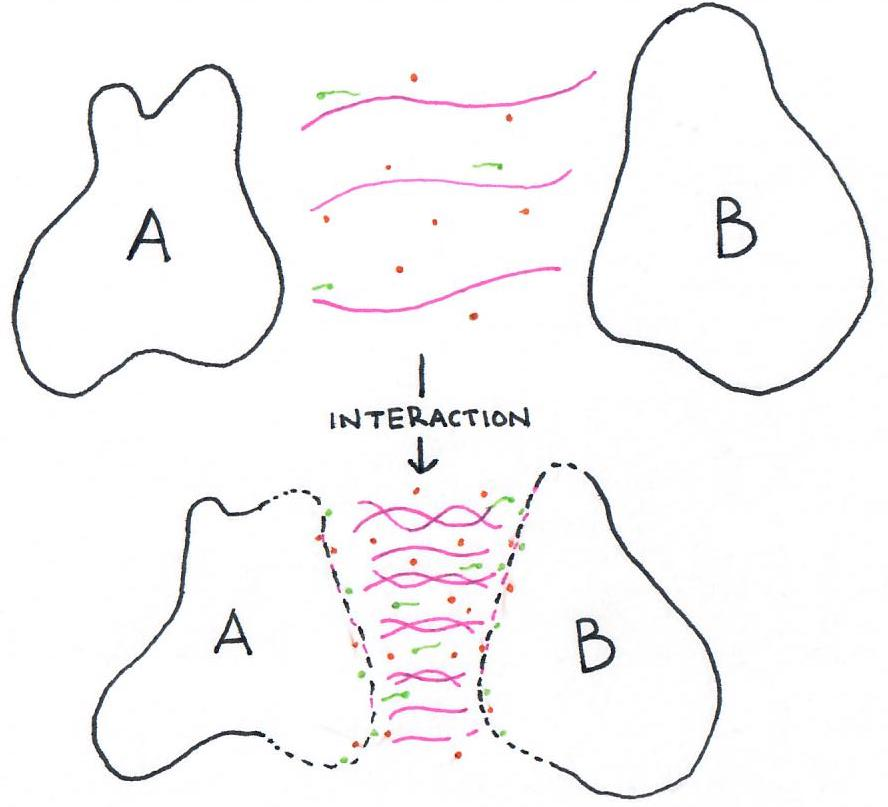
\includegraphics[width=0.5\textwidth]{interaction.jpeg}
		\caption{Two interacting systems}\label{fig:interacting-systems}
	\end{center}
\end{figure}


\subsection{Resource Theories}
When I think of resources I would normally think about something used to build another thing. Maybe concrete blocks are a resource for building new housing, or wood is a resource to heat your home. Point is, we often think of resources in terms of physical objects, but there is no need to restrict ourselves in this way. In fact one might think of brainpower as being a resource that is used by science to create new understanding. In this way, what we're doing is trying to understand how resources change, and in what ways they are allowed to change. As much as mathematicians and physicists may like it, you can't turn brainpower into coffee.

In fact, mathematical theories have already been constructed~\cite{mathematical-resources,resource-theory} for studying such ideas and (as the title of this section might hint to) are called \textbf{resource theories}. While the formal construction is quite complicated using ``symmetric monoidal categories'', the ideas are quite simple. In particular the na\"\i ve questions we might want to ask are
\begin{itemize}
	\item how do resources change during allowed processes?
	\item what are the allowed processes?
\end{itemize}
Or, put differently, what are the dynamics of our resources? These questions are encapsulated by category theory because of the way arrows (changes) and composition of arrows is built into categories.

Turning out eye to emerging quantum technologies, it might not be so clear how we can actually apply this resource theoretic framework to our field. But again we are thankful to those who have come before us developing quantum resource theories~\cite{quantum-resources} where the main quantum resources we have a coherence, and entanglement. What this means is that we are viewing coherence and entanglement as resources, and using these theories we can study how they change during allowed processes.

\subsection{Density Matrices}\label{sec:density-matrices}
Just briefly let's recall some facts about the density matrix that will be helpful in understanding this paper.
\begin{definition}
	Given a basis $\{\ket{\psi_n}\}$ for a Hilbert space $\mathcal{H}$, and corresponding probabilities $\{p_n\}$ for a state to be state $\ket{\psi_n}$, then the \textbf{density matrix} is given by
	\begin{equation*}
		\rho = \sum_n p_n\ketbra{\psi_n}.
	\end{equation*}
\end{definition}
The operator/matrix $\rho$ as defined above will always be positive semi-definite\footnote{$\bra{\phi}\rho\ket{\phi}\geq 0$ for all $\ket{\phi}\in\mathcal{H}$.}, Hermitian\footnote{$\rho^\dagger = \rho$.}, and have trace equal to 1\footnote{$\tr\rho = 1$.}. These three properties follow immediately from the above definition, along with the fact that the $p_n$ are probabilities and hence must sum to 1. Lastly recall that if we have an observable $\hat{A}$, then the expectation value with respect to a mixed state $\rho$ is given by $\overline{A} = \tr(\rho\hat{A})$.

\subsection{Entropy}
The paper is called ``The dynamics of entropies at the onset of interactions'', so it's probably best if we have a good understanding of what the authors mean by entropy.

Let's start with an arbitrary mixed state $\rho$. Because $\rho$ has trace 1, we know $\tr\rho^2\leq 1$ with equality holding if and only if $\rho$ is not in fact mixed, but a pure state $\rho = \ketbra{\psi}$. With this we can define a simple notion of ``purity'' by $\gamma = \tr\rho^2$. If $\rho$ represents an $n$ dimensional system, then $\gamma$ must fall in the range $\gamma\in\qty[\frac{1}{n}, 1]$ where the lowest values represent states that are more mixed, and higher values correspond to states that are more pure. We might also say this as states which are very likely in a handful of pure states.

A more sophisticated measure of purity or mixedness coming from (classical) information theory would be the Shannon/von Neumann entropy:
\begin{equation*}
	S(\rho)\coloneqq -\tr(\rho\ln\rho).
\end{equation*}
This measure does have the advantage of having an information theoretic backing, but in practice it is much harder to work with and calculate because of the logarithm.

Finally, there is one more notion we must introduce which is used in the paper. That of $n$-R\'enyi entropies, which can be defined as follows.
\begin{equation*}
	H_{n, B}(\rho)\coloneqq \frac{1}{1-n}\log(\tr_B\qty[\qty(\tr_A \rho)^n]) = \frac{1}{1-n}\log(\sum_i\lambda_i^n)
\end{equation*}
Where $\lambda_i$ are the eigenvalues of $\rho$. While it seems these entropies are not as frequently used, they provide a unifying framework for common entropies one does care about. In fact we have the max-entropy when $n = 0$, the min-entropy when $n\to\infty$, and the Shannon/von Neumann entropy when $n \to 1$.


\section{Main Results}

Why would we want a ``resource'' theory?
What are they good for?
What are our resources in quantum mechanics?
quantum things are really hard to control
introduce coherence
what does that mean mathematically?
- density matrix
- diagonal vs off diagonal elements
- 2-norm coherence?
as a resource, we'd like to understand the dynamics partially because it's interesting, but also because we can then better manipulate the resource



\subsection{2-Norm Coherence}
In this section we work through the calculations presented in section 2 of~\cite{dynamic-entropies}.
Let's start with showing the 2-norm coherence $\twonorm{}$ is the sum of the off diagonal elements squared of $\rho$.
To start, let's calculate the effect of the identity minus the dephasing operator $\dephase$ on our mixed state $\rho$.
It's important to note here that the dephasing operator (as the subscript might suggest) depends entirely on the operator $B$, because there is always a basis where $\rho$ is diagonal, and hence $\mathcal{D}_\rho\rho = \rho$.
\begin{equation*}
	\qty(\mathbb{1} - \dephase)\rho = \mqty[\rho_{11} & \rho_{12} & \cdots & \rho_{1d} \\ \rho_{21} & \rho_{22} & & \\ \vdots & & \ddots & \\ \rho_{d1} & & & \rho_{dd}] - \mqty[\diagonalmatrix{\rho_{11},\rho_{22},\ddots,\rho_{dd}}] = \mqty[0 & \rho_{12} & \cdots & \rho_{1d} \\ \rho_{21} & 0 & & \\ \vdots & & \ddots & \\ \rho_{d1} & & & 0] \eqqcolon \tilde{\rho}
\end{equation*}
Now we need to calculate the norm of this operator $\tilde{\rho}$ using the following norm definition $\norm{X}_2 \coloneqq \sqrt{\tr(X^\dagger X)}$.
Using the property the property that density matrices are Hermitian referenced in \cref{sec:density-matrices} we can simplify this as $\norm{\tilde{\rho}}_2 = \sqrt{\tr(\tilde{\rho}^2)}$.
Now we can calculate the diagonal elements of $\tilde{\rho}^2$ so we can sum them up and get the trace.
\begin{equation*}
	\tilde{\rho}^2 = \mqty[0 & \rho_{12} & \cdots & \rho_{1d} \\ \rho_{21} & 0 & & \\ \vdots & & \ddots & \\ \rho_{d1} & & & 0]^2  = \mqty[\dmat{\sum_{i \neq 1 }^d\rho_{1i}\rho_{i1},\sum_{i \neq 2}^d\rho_{2i}\rho_{i2},\ddots, \sum_{i \neq d}^d\rho_{di}\rho_{id}}]
\end{equation*}
This expression, with the fact that $\rho_{ij} = \overline{\rho_{ji}}$ allows us to write the trace, and hence the 2-norm coherence as
\begin{equation}\label{eq:2norm}
	\twonorm{} \coloneqq\norm{\qty(\mathbb{1} - \dephase)\rho}_2^2 = \sum_{\substack{i\neq j \\ i,j = 1}}^d\abs{\rho_{ij}}^2.
\end{equation}
The fact that we are representing $\rho$ in the eigenbasis of $B$ rather than the ``natural'' basis of $\rho$ where it is diagonal means $\rho$ \emph{is} likely to have off-diagonal elements in the first place. I mention this because I've only ever worked with density matrices in the most ``natural'' bases where things are quite simple.

\begin{example}\label{ex:qubits}
	To get an idea how some of this machinery is working, let's work with one of the simplest examples: a qubit. This means both our observable $B$ and density matrix $\rho$ are $2\times 2$ matrices, and in particular we can write $B$ as
	\begin{equation*}
		B = b_x\ketbra{b_x} + b_y\ketbra{b_y} = \mqty[b_x & 0 \\ 0 & b_y].
	\end{equation*}
	Where $b_x$ and $b_y$ are the eigenvalues of $B$ corresponding to eigenvectors $\ket{b_x}$ and $\ket{b_y}$. In this basis we can then write down an arbitrary density matrix as
	\begin{equation*}
		\rho = \sum_{i, j\in \{x, y\}}\rho_{ij}\ketbra{b_i}{b_j} = \mqty[\rho_{xx} & \rho_{xy} \\ \rho_{yx} & \rho_{yy}].
	\end{equation*}
	With these in place we can now calculate the variance of $B$ as follows.
	\begin{align*}
		(\Delta B)^2 & \coloneqq \overline{B^2} - \overline{B}^2 = \tr(\rho B^2) - \qty[\tr(\rho B)]^2                                        \\
		             & = \tr(\mqty[\dmat{\rho_{xx}b_x^2, \rho_{yy}b_y^2}]) - \qty[\tr(\mqty[\dmat{\rho_{xx}b_x, \rho_{yy}b_y}])]^2            \\
		             & = \rho_{xx}b_x^2 + \rho_{yy}b_y^2 - \rho_{xx}^2b_x^2 - 2\rho_{xx}\rho_{yy}b_x b_y - \rho_{yy}^2b_y^2                   \\
		             & = \rho_{xx}b_x^2 + (1 - \rho_{xx})b_y^2 - \rho_{xx}^2b_x^2 - 2\rho_{xx}(1 - \rho_{xx})b_x b_y - (1 - \rho_{xx})^2b_y^2 \\
		             & = \rho_{xx}\qty(b_x^2 + b_y^2 - 2b_x b_y) - \rho_{xx}^2\qty(b_x^2 + b_y^2 - 2b_x b_y)                                  \\
		             & = \qty(\rho_{xx} - \rho_{xx}^2)\qty(b_x - b_y)^2
	\end{align*}
	Further, we can actually show that we can write this using both the purity $\gamma\coloneqq\tr(\rho^2)$ and the 2-norm coherence defined in \cref{eq:2norm}.
	\begin{align*}
		\frac{1 - \gamma + \twonormE}{2} & = \frac{1}{2}\qty(1 - \tr(\rho^2) + \twonormE)                                             \\
		                                 & = \frac{1}{2}\qty(1 - \rho_{xx}^2 - \rho_{yy}^2 - 2\abs{\rho_{xy}}^2 + 2\abs{\rho_{xy}}^2) \\
		                                 & = \frac{1}{2}\qty(1 - \rho_{xx}^2 - \rho_{yy}^2)
	\end{align*}
	Note here that the $\rho_{ii}$ terms don't need an absolute value because diagonal terms of the density matrix are always real by the Hermiticity condition $\rho_{ii} = \overline{\rho_{ii}}$.
	We can now use the fact that $\tr\rho = 1$ to write $\rho_{yy} = 1 - \rho_{xx}$ to rewrite our equation purely in terms of $\rho_{xx}$.
	\begin{equation*}
		\frac{1 - \gamma + \twonormE}{2} =\frac{1}{2}\qty(1 - \rho_{xx}^2 - \qty[1 - 2\rho_{xx} + \rho_{xx}^2]) = \rho_{xx} - \rho_{xx}^2
	\end{equation*}
	In total, this allows us to write the variance of an observable $B$ as
	\begin{equation*}
		(\Delta B)^2 = \frac{1 - \gamma + \twonormE}{2}\qty(b_x - b_y)^2.
	\end{equation*}
	The maximally mixed state $\rho = \frac{1}{N}\mathbb{1}$ has purity $\gamma = \frac{1}{N}$, or in our case where $N = 2$, $\frac{1}{2}$. This state possess no off diagonal elements, so conveniently $\twonorm{\rho} = 0$. These observations define $(\Delta B)_\text{max}^2 = \frac{1}{4}\qty(b_x - b_y)^2$. As in~\cite{dynamic-entropies} we can then write
	\begin{equation}\label{eq:variance-max}
		\frac{(\Delta B)}{2(\Delta B)_\text{max}^2} = \twonormE + \mu
	\end{equation}
	where $\mu\coloneqq 1 - \gamma$ is the ``mixedness'' of a state. \Cref{eq:variance-max} shows us that we can think of the variance as composed of two pieces: one which quantifies how much classical uncertainty a state has, and one which quantifies coherent superposition.
\end{example}

\subsection{2-Fragility}
In equation (26) of~\cite{dynamic-entropies} the 2-fragility is given to be
\begin{equation}\label{eq:2fragility}
	f_2 = -\frac{1}{2}\tr_B\qty(\comm{B}{\rho_{B, 0}}^2)
\end{equation}
whereas the general definition of the $n$-fragility is given by
\begin{equation}\label{eq:nfragility}
	f_n\coloneqq -\frac{n}{2}\tr_B\qty(\rho_{B, 0}^{n-1}\comm{B}{\rho_{B, 0}}B).
\end{equation}
We first show that $f_2$ can be written as \cref{eq:2fragility} starting from the definition given in \cref{eq:nfragility}.
\begin{align*}
	f_n & \coloneqq -\tr_B\qty(\rho_{B, 0}\comm{B}{\rho_{B, 0}}B)                                                                                                         \\
	    & = -\tr_B\qty(\rho_{B, 0}B\rho_{B, 0}B - \rho_{B, 0}^2B^2)                                                                                                       \\
	    & = -\frac{1}{2}\tr_B\qty(\rho_{B, 0}B\rho_{B, 0}B + \rho_{B, 0}B\rho_{B, 0}B - \rho_{B, 0}^2B^2 - \rho_{B, 0}^2B^2)                                              \\
	    & = -\frac{1}{2}\tr_B\qty(\rho_{B, 0}B\rho_{B, 0}B + B\rho_{B, 0}B\rho_{B, 0} - \rho_{B, 0}B^2\rho_{B, 0} - B\rho_{B, 0}^2B) \tag{\footnotesize{cyclic property}} \\
	    & = -\frac{1}{2}\tr_B\qty(\comm{\rho_{B, 0}}{B}^2)
\end{align*}
It's worth noting that this identity does not hold for any other $n$. In fact the identity only holds here because $2+2 = 2\cdot 2$. To see this notice the terms in $\rho^{n-1}\comm{B}{\rho}B$ are multiplications of $n+2$ elements\footnote{For example if $n = 3$ we have $\rho^{2}\comm{B}{\rho}B = \rho^2B\rho B - \rho^3B^2$, and hence each term consists of 5 pieces (even if some might be redundant).}, whereas $\comm{\rho}{B}^n$ in general has elements that are multiplications of $2n$ elements.

\subsection{Interacting Systems}
In this paper there are two main types of interaction that are looked at. First, we have our system $B$ which is brought into contact/interaction with another ancillary system $A$. In full generality the Hamiltonian for this system would be
\begin{equation*}
	H = H^{(A)}_\text{free}\otimes\mathbb{1} + \mathbb{1}\otimes H^{(B)}_\text{free} + H^{(AB)}_\text{interaction}.
\end{equation*}
This paper makes the simplifying assumption that the we're working in the regime where the interaction is completely dominant, and the free terms can be neglected. Further that the interaction term can be written as $H_A\otimes H_B$ where $H_A$ and $H_B$ are some operators acting one a single system. The first type of interaction looked at are interactions where $H_A = A$ and $H_B = B$ where $A, B$ are self-adjoint operators.

In this first case the time evolution operator will be $U(t) = \e^{\iu tA\otimes B}$, and we'll first start with a little detour to show a simple fact that will be very handy.

\subsubsection{Commuting with the time evolution operator}\label{sec:commuting-with-time}
As is often discussed in quantum mechanics class, when something commutes with the Hamiltonian, that implies something is constant in time. This goes back to Hamilton's equation which states for a time independent Hamiltonian $H$, and observable $f$ the time evolution is given by
\begin{equation*}
	\dv{f}{t} = \pb{f}{H}.
\end{equation*}
In the quantum case the Poisson bracket takes the form $\pb{-}{-}\to\frac{1}{\iu\hbar}\comm{-}{-}$. Thus we see if something commutes with the Hamiltonian, then it must be constant in time. A direct result of this is that the variance $\Delta f(t)$ is independent of time, and hence $\dv{t}\Delta f(t) = 0$. That said, in~\cite{dynamic-entropies} the authors use the fact that an operator $\mathbb{1}\otimes B$ commuting with the \textbf{time evolution operator} of the form $U(t) = \e^{\iu t A\otimes B}$ \emph{also} implies $\dv{t}\Delta B(t) = 0$. This is not complicated, but non-trivial, and so we'll go through the steps to show that here.
\begin{align*}
	\qty(\mathbb{1}\otimes B)U(t) & = \qty(\mathbb{1}\otimes B)\sum_{n = 0}^\infty\frac{(\iu t)^n}{n!}\qty(A\otimes B)^n                                  \\
	                              & = \sum_{n = 0}^\infty\frac{(\iu t)^n}{n!}\qty(\mathbb{1}\otimes B)\qty(A^n\otimes B^n)                                \\
	                              & = \sum_{n = 0}^\infty\frac{(\iu t)^n}{n!}\qty(A^n\otimes B^{n+1})                                                     \\
	                              & = \sum_{n = 0}^\infty\frac{(\iu t)^n}{n!}\qty(A\otimes B)^n\qty(\mathbb{1}\otimes B)  = U(t)\qty(\mathbb{1}\otimes B)
\end{align*}
Now this manipulation does not prove that commuting with the Hamiltonian \emph{always} implies an observable will commute with the time evolution operator, but the above can be applied to an arbitrary Hamiltonian $H$ that is time independent. Also it seems like this technically proves $\dv{t}\Delta(\mathbb{1}\otimes B) = 0$, but surely we can make the identification of this without the tensor product with the identity.

So now we know $\Delta B$ is constant, and by~\cref{eq:variance-max} we can see $\twonormE + \mu = \text{constant}$. So in this case when entanglement goes up, we lose coherence and vice versa. This is a great result, but bad for us since most of the time we want both coherence \emph{and} entanglement when working with quantum technologies.

In the second case, we take $H_A = A$ as before, but now we take $H_B$ to be some arbitrary operator that \emph{does not} commute with $B$. This disallows the manipulation we went through in \cref{sec:commuting-with-time}, so we should expect this to be more complicated. Indeed the situation is, and the important finding is that it's actually possible to both increase coherence and entanglement \emph{at the same time} contrary to what I would have expected\footnote{It seems if we could figure out how to harness this, it would be a major win!}.

\section{Conclusion}

In this summary we've tried to highlight the best, and most interesting pieces of the paper \emph{The Dynamics of Entropies at the Onset of Interactions}~\cite{dynamic-entropies}. We started out by motivating why one might care about the exchange of quantum resources during processes like quantum computation and quantum communication. In particular to better understand the interactions of quantum systems, but also so we can build more effective technology harnessing these powers.

We then introduced some key ideas needed to understand the ideas presented in the paper, and sequentially used them in \cref{ex:qubits} to show how we can dissect a systems variance into two pieces: one pertaining to classical ignorance, and one describing a systems coherence superposition\footnote{How much of a stretch would it be to call this the quantum ignorance? It might just be the symmetry appealing to me, but it does feel like ``quantum ignorance'' isn't a bad way to describe superposition.}.

\subsection{Questions}
When working with a the time evolution operator of the form $U(t) = \e^{\iu tA\otimes H_B}$ we take
\begin{equation*}
	H_B \coloneqq -\iu\qty(\ketbra{b_x}{b_y} - \ketbra{b_y}{b_x}) = -\iu\mqty[0 & 1 \\ -1 & 0] = \mqty[0 & -\iu \\ \iu & 0] = \sigma_y.
\end{equation*}
I was confused here because we're using $\sigma_x$, which I'm assuming denotes the first Pauli matrix $\mqty[0 & 1 \\ 1 & 0]$, but then define the operator $H_B$ in a way that obscures the fact that it's the second Pauli matrix.

\subsection{Applications}

Before we end, I'm left with lots of ideas and questions about where this work might apply to.

\subsubsection{Quantum Embezzlement}
``Quantum embezzlement'' described in~\cite{embezzlement,self-embezzlement}, is a process that allows one to use a catalyst state to clone a quantum state in a way that does not violate the no-cloning theorem. This process is extremely interesting because it not only goes against a fundamental theorem in the field of quantum information, but it provides a new mechanism for doing something once thought impossible. I would be very much interested in learning more about how our existing quantum resource theories can be made to fit with these new finding (or it's possible there are no existing contradictions). Even viewing this process of embezzlement from a resource theoretic perspective would be very interesting.

As a more direct application of this paper, I would be interested in finding out how the two interacting states in the embezzlement process exchange coherence and entanglement using methods derived in~\cite{dynamic-entropies}. The fact that there is a catalyst state that remains unchanged (physically undetectable at least) through the protocol I would expect that some of it's entanglement is siphoned off and ``given'' to embezzling state. That said of course it would be important to prove or disprove these conjectures, and I think the tools developed here could shed light on the process.

\subsubsection{Quantum Error Correction}
As we know, maintaining coherence in a quantum computer is extremely challenging. Since some of the original work in~\cite{error-correction}, we have seen many new methods and protocols for doing quantum error correction. It would be very interesting to study some of these methods to see how measures of entanglement and coherence change throughout some given circuits. I understand the circuit model of quantum computation is quite different from that of the Hamiltonian model used in this work, but I believe the two are equivalent, and so it should be possible.

\clearpage

\bibliography{refs}

\end{document}